Generally the design of the user interface for the web application is an integration of the principles previously described with core design elements of web and the twitter bootstrap element library.

The web client use a bootstrap styled navigation bar for main navigation where the navigation tabs look more like links in a web navigation bar. There are three types of views in the web client:

\begin{itemize}
	\item \textbf{Main views:} A main view covers the entire page. The structure among main views is shallow and the user may freely navigate between all main views using the navigation bar. Search and navigation are main views.
	\item \textbf{Sub views:} A main view may consist of several sub views. In this case the main view has a vertical navigation bar on the left side used to navigate between sub views, sub views may not be directly navigated outside of its main view. The user may navigate to other main views from a sub view. Except for the sub navigation bar the sub view covers the entire main view, replacing its content. There are sub views in the administration main view.
	\item \textbf{Modal views:} Modal views “rolls over” the current main view and are used for specialized operations. Modal views can navigated to using buttons inside main views and sub views. Usually the user will be taken back to the previous view when the modal is closed but navigation in a sequence of modal views could be implemented in the future. Processing of raw files is currently done in a modal view.
\end{itemize}

Content that belong together is grouped using so called "panels", a header that describes the content with an area for the content below, with everything wrapped up by a border.
The contrast between elements in the interface is of medium strength. Grayscale colors are used for most elements but elements that need to be highlighted or distinguished from other elements use colors. Colors with high saturation are used for highlighting and colors used for distinguishing elements have a lower saturation.

Buttons that perform actions always contain an icon and text so that the experienced user may more quickly perform the desired actions but finding buttons at a glance instead of reading button text.

\subsubsection{Search view}
The search view consists of two main parts, at the top there is a group of buttons for performing actions on files and experiments. This button group also contains the search query input and search button.

Below is a table where search results are shown. The table consists of different types of rows:

\begin{itemize}
	\item Experiment rows: These rows represent an experiment, they can be expanded to reveal the files contained in an experiment. The row has columns for the expand button, the experiment name and the annotations.
	\item File type rows: When an experiment is expanded three new rows are expanded, each representing one type of file. They can be expanded to reveal the files of that type that belong to the experiment. File column headers are also shown when a file row is expanded.
	\item File rows: These rows represent the files existing in an experiment. They have a checkbox that can be checked to select the file so that it can be used by the various actions exposed in the button group. File rows also have columns for file data.
\end{itemize}

\subsubsection{Upload view}
\begin{figure}[h]
\centering
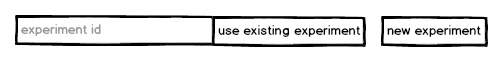
\includegraphics[width=1\textwidth]{web_id_uploadFields.png}
\caption{\label{fig:web_id_uploadFields}Fields for experiment selection/creation.}
\end{figure}

The upload view has two states, first the user have to choose if it wants to create a new experiment to upload files or use an existing file. This step looks like \refer{fig:web_id_uploadFelds}.

\begin{figure}[h]
\centering
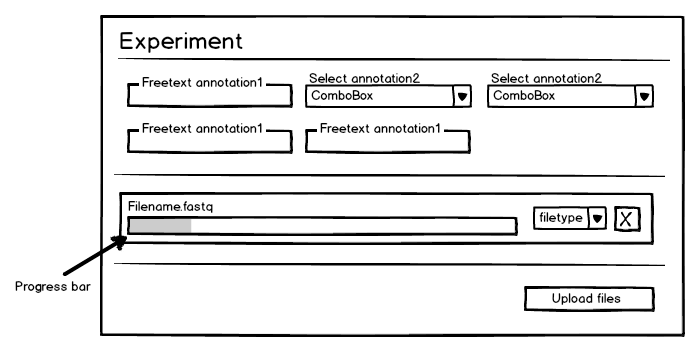
\includegraphics[width=1\textwidth]{web_id_fileUpload.png}
\caption{\label{fig:web_id_fileUpload}File upload and experiment annotation view.}
\end{figure}

Once the user has an experiment to upload files to it may start to upload files and annotate the experiment. The step for doing that looks like \refer{fig:web_id_fileUpload}.

\subsubsection{Process view}
The process view has a set of input and select fields for the user to input parameters to be used in the file processing. At the bottom of the view there’s a button used to start the processing.
